\documentclass[times, utf8, zavrsni, numeric]{fer}
\usepackage{booktabs}
\usepackage{listings}
\usepackage{color}
\usepackage{url}
\usepackage{amsmath}


%Engleski termini
\newcommand{\eng}[1]{(eng. \textit{#1})}

\begin{document}

\title{ Lokalizacija karakterističnih točaka lica u videu }

\author{ \begin{tabular}{ l }
	Generalić Boris \\
	Gulan Filip \\
	Kopljar Damir \\
	Miličević Andrija \\
	Nuić Hrvoje \\
	Šarić Fredi \\
	Zadro Tvrtko \\
\end{tabular}  }

\maketitle
\tableofcontents

\chapter{Projektni zadatak}

\section{Opis projektnog zadatka}

Lokalizacija karakterističnih točaka lica u videu ili fotografiji je tehnika koja se danas koristi u mnogim sustavima i uređajima. Susrećemo je na raznim društvenim servisima, poput \textit{Facebook-a}, koji ju koriste za automatsko označavanje ljudi na fotografijama. Većina algoritama lokalizacije točaka lica su iznimno kompleksni i zahtijevaju veliku količinu procesorske snage i memorije, pa je težnja usmjerena na poboljšavanje tih algoritama. No razvojem i napretkom tehnologije algoritmi lokalizacije točaka lica se danas uspješno, bez velikih problema, izvode i na mobilnim uređajima koji ih koriste u raznoraznim aplikacijama poput alata za šminkanje gdje osoba može uz pomoć praćenja lica vidjeti kako bi izgledali s određenim bojama na svom licu.

Kroz ovaj projekt će se pokušati dani problem lokalizacije karakterističnih točaka lica riješiti uporabom dubokih neuronskih mreža.

\section{TODO: Pregled i opis srodnih rješenja}

Iscrpan pregled srodne literature s predloženim rješenjima. Opis postojećih ispitnih baza (linkovi na javno dostupne baze).

\section{Konceptualno rješenje zadatka}

Sam sustav za lokalizaciju karakterističnih točaka lica je podijeljen u više segmenata, tj. podsustava. Prvi segment sustava na ulaz prima sliku ili jedan vremenski okvir video isječka. Dana slika ili isječak se zatim pretvaraju u sliku sivih nijansi. Tako obrađena slika se dovodi na ulaz podsustava za izlučivanje položaja svih lica na slici te kao rezultat vraća listu u obliku: koordinate gornjeg lijevog ugla, širina i visina lica.

Tako dobivena lista se zatim iskoristi na način da se iz slike sivih nijansi izrežu prepoznata lica i skaliraju. Pojedina skalirana lica dovede se na ulaze duboke neuronske mreže koja kao izlaze daje koordinate odabranih karakterističnih točaka lica. Tako dobivene točke skaliraju se u prostor početne slike ili isječka te se iscrtavaju i prikazuju korisniku sustava.

\chapter{Postupak rješavanja zadatka}

\section{Pretvorba boje u nijanse sive}

Prvi korak koji je potrebno napraviti na ulaznoj slici je pretvoriti ju u sliku sivih nijansi. Kod prikaza boja slike korištenjem aditivnog RGB \engl{Red Green Blue} modela postoje tri komponente: crvena, zelena i plava. Kombinacijom te tri komponente u različitim omjerima dobivamo ostale boje. Da se uočiti da podjednakom raspodjelom svih triju komponenti dobivamo boje iz sivog spektra, pa se algoritam pretvorbe u sliku sivih nijansi temelji na odabiru jedne vrijednosti iz dane tri komponente kako bi se dobila siva nijansa.

\subsection{Prvi algoritam}

Prvi algoritam je vrlo jednostavan i intuitivan. Siva nijansa pojedinog slikovnog elementa se dobiva tako da se boja slikovnog elementa rastavi na tri navedene komponente. Omjer pojedinih komponenti se zbraja te se uzima srednja vrijednost, kako je prikazano izrazom \eqref{eq:ug}.
\begin{equation}\label{eq:ug}
E_y = \frac{E_R + E_G + E_B}{3}
\end{equation} 

\subsection{Drugi algoritam}

Prvi algoritam je intuitivan i vrlo jednostavan, no u praksi ne daje najbolje rezultate. Problem leži u ljudskom oku i načinu na koji opaža boje. Ljudsko oko zelenu boju opaža puno jače nego crvenu, te crvenu opaža jače nego plavu. Stoga intuitivno slijedi da bi zelena trebala biti najzastupljenija, zatim crvena i plava. Organizacija ITU \engl{International Telecommunication Union} u svojoj normi ITU-R BT.709-6 \citep{ITUgrayscale} predlaže drugi algoritam u kojem bi crvena komponenta imala udio s 22.16\%, zelena s 71.56\% te plava s 7.22\%, što je prikazano izrazom \eqref{eq:itu_grayscale}.
\begin{equation} \label{eq:itu_grayscale}
E_y = 0.2126E_R + 0.7152E_G + 0.0722E_B
\end{equation}

Na slici \ref{fig:grayscale_example_all} mogu se usporediti rezultati obadva izraza, gdje je jasno vidljiva prednost korištenja izraza \eqref{eq:itu_grayscale}.

\begin{figure}[htb]
    \centering
    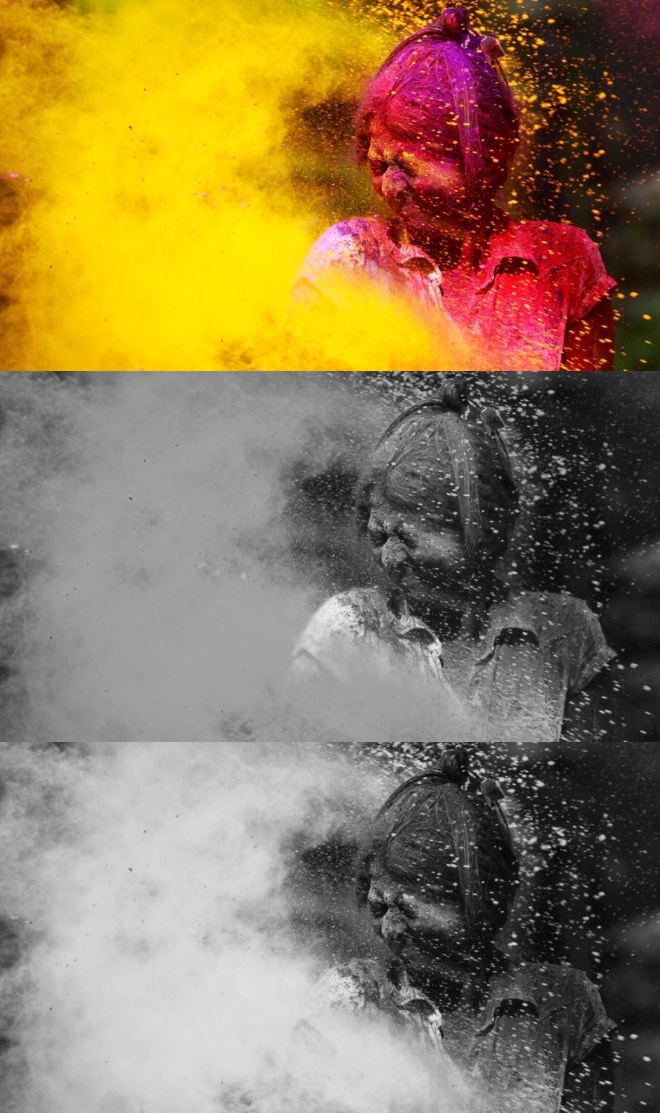
\includegraphics[width=9cm]{images/grayscale_example_all.jpg}
    \caption{Usporedba prvog i drugog algoritma pretvorbe boja u nijanse sive}
    \label{fig:grayscale_example_all}
\end{figure}

\section{Izjednačavanje histograma}

Nakon što je slika u boji pretvorena u sliku sivih nijansi vrlo lako je moguće da kontrast na danoj slici nije najbolji. U namjeri poboljšanja kontrasta na slici te izoštravanja pojedinih elemenata koristi se izjednačavanje histograma.

Izjednačavanje histograma slike je operacija pri kojoj se slika mijenja tako da broj točaka za pojedinu nijansu sive bude približno jednoliko raspoređen. Matematički rečeno izjednačavanje histograma implicira preslikavanje početne distribucije na širu i "uniformniju" distribuciju.

Kako je za potrebe ovog projekta korištena biblioteka \emph{OpenCV}, za izjednačavanje histograma korištena je metoda \emph{equalizeHist} iz navedene biblioteke. Primjer rada algoritma vidljiv je na slici \ref{fig:eq_hist}.

\begin{figure}[htb]
    \centering
    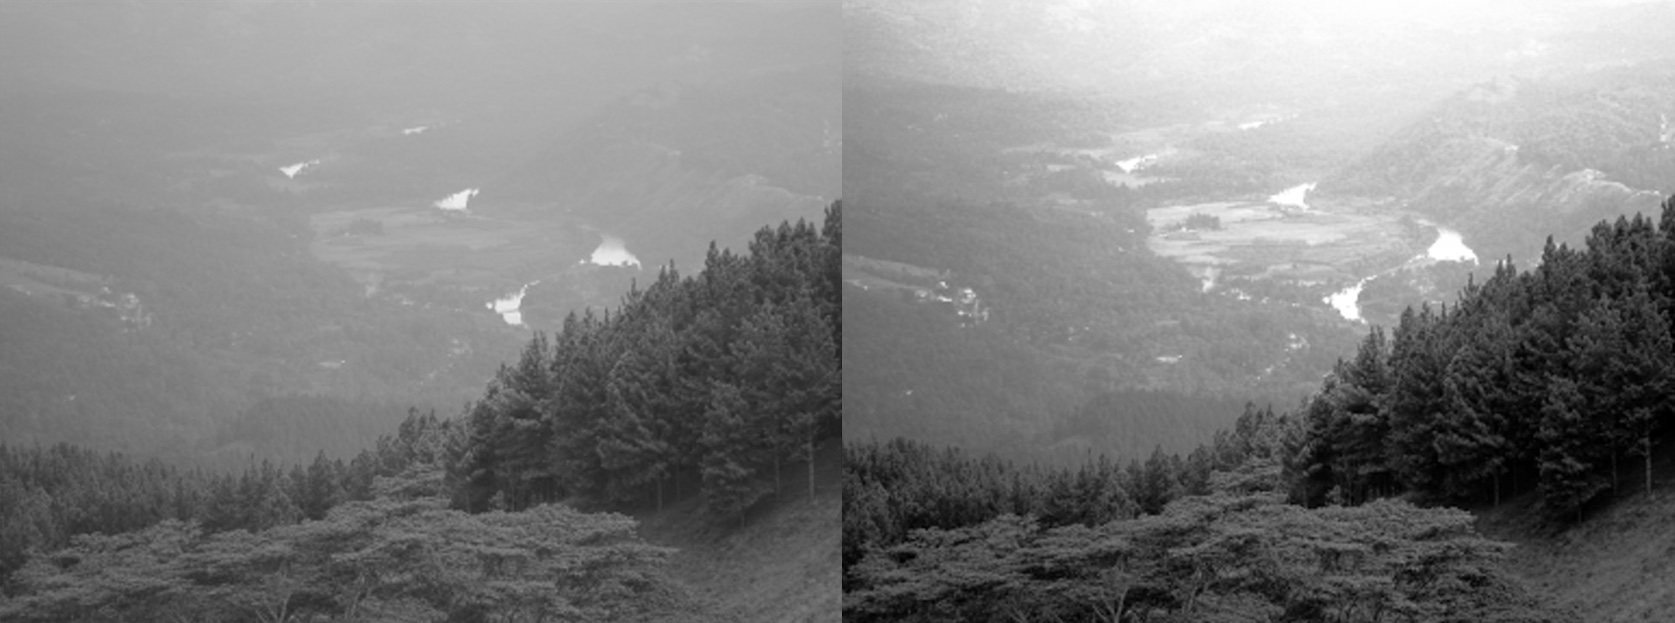
\includegraphics[width=14cm]{images/eq_hist.jpg}
    \caption{Izjednačavanje histograma}
    \label{fig:eq_hist}
\end{figure}

\section{Detekcija i izlučivanje lica}


\chapter{Ispitivanje rješenja}
(do 10 stranica)

\section{Ispitna baza}
Opisati ispitnu bazu, tipove i broj različitih uzoraka u bazi te na koji su način uzorci iz baze korišteni prilikom učenja i ispitivanja rješenja projektnog zadatka. 

\section{Rezultati učenja i ispitivanja}
Prikazati statističke podatke o uspješnosti rješenja prilikom učenja/ispitivanja te opisati eksperimente na temelju kojih su podaci dobiveni.

\section{Analiza rezultata}

Analizirati uzroke rezultata ispitivanja, povezati sa uzorcima u bazi i algoritmima korištenim u rješenju. Raspraviti moguća poboljšanja.

\chapter{Opis programske implementacije rješenja}

Opisati sučelje programske implementacije i način korištenja implementacije.


\chapter{Zaključak}

(do 2 stranice)

Ocijeniti uspješnost implementacije, navesti budući rad u smislu potrebnih poboljšanja. 

\bibliography{literatura}
\bibliographystyle{fer}

\end{document}
